This chapter is aimed to give a basic introduction to the \textbf{Aerospace applications} part of this course, whose focus will be particularly on spacecraft and more specifically \textbf{satellites}.

\begin{figure}[h]
    \centering
    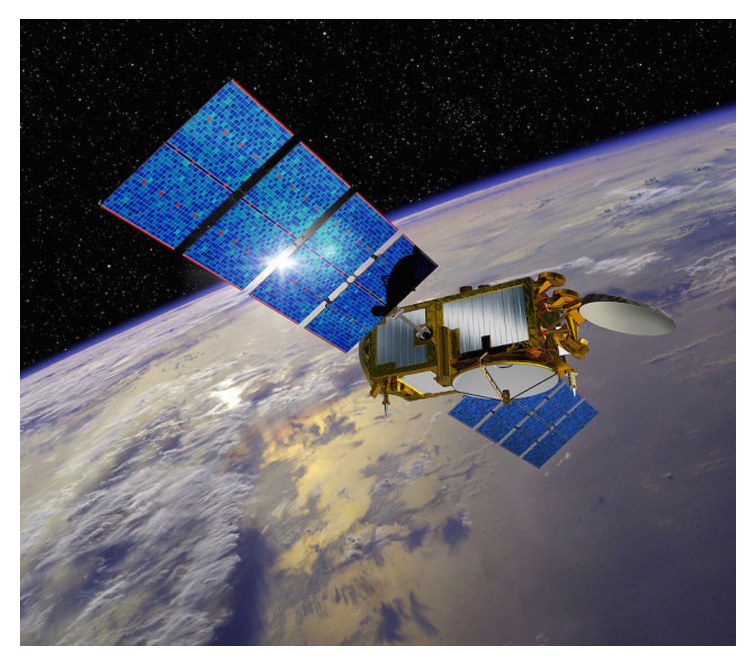
\includegraphics[scale=0.7]{AerospaceApplications/images/satellite_img.png}
    \caption{A satellite on MEO}
\end{figure}

There are many fields in which satellites are used: Earth observation, scientific research, ICT field, other planet observation and so on.\\
Their size is very variable: from few chilos to many tons. During its life a satellite can: reaching a target orbit for a mission for example otherwise a satellite can be exploited to check out some space instrumentation.\\

A satellite can work in one of the three types of orbit. The orbits can be classified in: 
\begin{itemize}
    \itemsep0em
    \item Low Earth Orbit \textbf{(LEO)}: 180-2000 km (above the Earth surface)
    \item Medium Earth Orbit \textbf{(MEO)}: 2000-35000 km
    \item Hight Earth Orbit \textbf{(HEO)}: $\ge$35000 km
\end{itemize}

The topics of this part are divided in this way: 
\begin{enumerate}
    \itemsep0em
    \item \textbf{Attitude dynamics and control}
    \begin{itemize}
        \itemsep0em
        \item rotations, attitude kinematics and dynamics
        \item attitude control
    \end{itemize}
    \item \textbf{Orbital dynamics and control}: 
    \begin{itemize}
        \itemsep0em
        \item orbital dynamics; 
        \item orbital control.
    \end{itemize}
\end{enumerate}

The first part of each chapter will be in order to introduce some theoretical aspect which are fundamental to understand and control a spacecraft. In the part reguarding the \textbf{spacecraft attitude} some results about mathematical tools for rotations are given.

